\section{Introduction}

In computing systems, performance and energy consumption are conflicting goals -- increasing performance requires a super-linear increase in power consumption.
Thermal design constraints limit both the maximum and average performance that a computing system can achieve.
Fortunately, modern systems expose knobs that allow hardware and software to trade performance and power/energy consumption, so that a desired balance can be reached.
For example, most systems provide a mechanism to control dynamic voltage and frequency scaling (DVFS), trading processor clock rate and power consumption for changes in throughput.
Another common approach is to change the allocation of the number of compute cores on multicore systems, allowing unallocated cores to enter low-power sleep states, or even shut down altogether to save power/energy.

We can characterize the performance and power consumption of applications in different system configurations by testing them in each configuration and recording the behavior.
Performance and power form a non-linear, convex tradeoff space, where each system configuration, \eg DVFS setting, produce a unique application performance and system power values.
% \TODO{Show an example.}

% In some cases, the goal is simply to run software as fast as possible, and as long as energy consumption is not a concern, this is acceptable.
As power and energy become first-class concerns in computing systems ranging from low-power embedded to large scale high-performance computing (HPC), there is an increasing need for software to manage hardware resource allocations to achieve a desirable balance in performance and power/energy consumption.
Heuristic approaches rely on assumptions about the performance/power tradeoff space of an application and system that we have found are not portable between applications and systems (as we demonstrated in embedded systems) \cite{Imes2014}.
For example, the classic race-to-idle heuristic can achieve low energy consumption on one system, but poor on another compared with an approach that never idles (or even a pace-to-idle approach).
An interesting observation by Kim \etal is, ``Unless the function of a given machine is a straight line originating from the idle state, (0, $P_{idle}$), an idling heuristic is never optimal for all instances'' \cite{kim-cpsna2015}.
The more convex the tradeoff space, the further from optimal any idling approach is.

\begin{figure}[t]
  \begin{centering}
  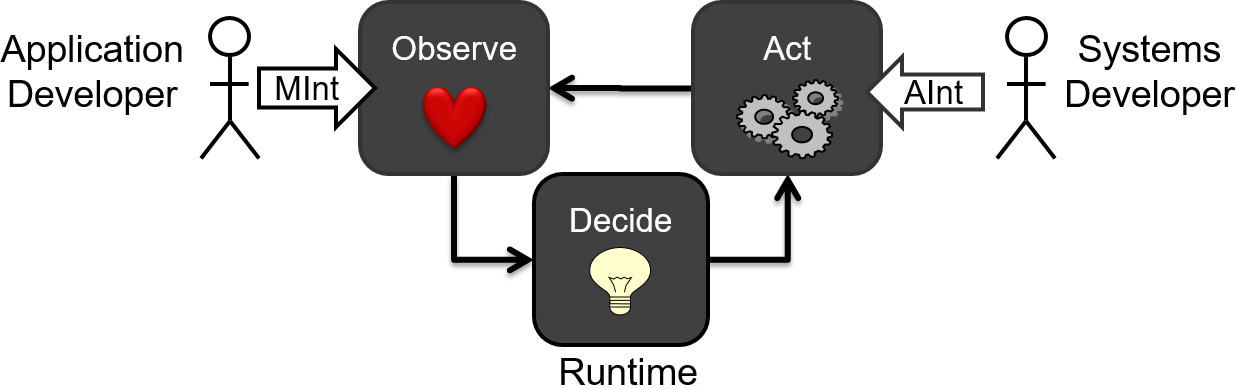
\includegraphics[width=0.6\textwidth]{figs/SEEC.png}
  \caption{A self-aware computing (SEEC) runtime model -- observe, decide, and act.}
  \label{fig:seec}
  \end{centering}
\end{figure}

The lack of both portability and optimality of heuristics demand that we develop more general approaches to addressing the problems in balancing performance and power.
In his PhD thesis, Hoffmann proposes a ``self-aware'' computing model (SEEC) that uses a closed-loop feedback design to ``observe, decide, and act'' \cite{HoffmannPhD}.
\figref{seec} demonstrates this concept.
The SEEC model is more portable than heuristics because it includes an observation step that measures behavior at runtime rather than relying strictly on assumptions made offline.
We build on this high-level model and use feedback systems that measure application and system behavior during runtime to make changes to resource allocations as new information becomes available.
Furthermore, the general design of our feedback systems, although still relying on some offline characterization of application and system behavior, are not dependent on extremely accurate or complete models, instead relying on runtime measurements to adapt.


This thesis addresses two common approaches in managing performance and power consumption.
The first approach is meeting an application performance goal while attempting to minimize the total energy consumption.
We formulate this as a constrained optimization problem, using control theory to meet the performance goal, and linear optimization to select the optimal pair of system configurations to use that satisfy the performance constraint.
This is practical since in the aforementioned work, Kim \etal prove that an optimal solution to this constrained optimization problem requires, at most, two configurations from the performance/power tradeoff space \cite{kim-cpsna2015}.
The second approach addresses the problem of running software as energy-efficiently as possible, \ie maximizing the ration of work completed to energy consumed.
By treating this as a classification problem, we can use samples from low-level hardware counters to drive well-understood machine learning approaches that predict the most energy-efficient configuration to use, without requiring the software to provide its own instrumentation.
